\documentclass[conference]{IEEEtran}
\IEEEoverridecommandlockouts
% The preceding line is only needed to identify funding in the first footnote. If that is unneeded, please comment it out.
\usepackage{cite}
\usepackage{amsmath,amssymb,amsfonts}
\usepackage{algorithmic}
\usepackage{graphicx}
\usepackage{textcomp}
\usepackage{hyperref}
\usepackage{booktabs}
\usepackage[table]{xcolor}
\usepackage{multirow}

\newcommand{\cho}[1]{{\color{red}{#1}}}

\def\BibTeX{{\rm B\kern-.05em{\sc i\kern-.025em b}\kern-.08em
    T\kern-.1667em\lower.7ex\hbox{E}\kern-.125emX}}
\begin{document}

\title{SPbLA: The Library of GPGPU-Powered Sparse Boolean Linear Algebra Operations
}

\author{
\IEEEauthorblockN{Egor Orachev}
\IEEEauthorblockA{\textit{Saint Petersburg State University} \\
%\textit{name of organization (of Aff.)}\\
\textit{JetBrains Research,} \\
St. Petersburg, Russia \\
egor.orachev@gmail.com}
\and

\IEEEauthorblockN{Maria Karpenko}
\IEEEauthorblockA{\textit{ITMO University} \\
%\textit{name of organization (of Aff.)}\\
St. Petersburg, Russia \\
mkarpenko.spb@gmail.com}
\and

% \IEEEauthorblockN{Vasily Kuporosov}
% \IEEEauthorblockA{\textit{HSE University} \\
% %\textit{name of organization (of Aff.)}\\
% St. Petersburg, Russia \\
% vvkuporosov@edu.hse.ru}
% \and

% Не бейте меня. Просто хотел места больше свободного сделать

\IEEEauthorblockN{Artem Khoroshev}
\IEEEauthorblockA{\textit{Computation Biology} \\
\textit{Department} \\
\textit{BIOCAD}\\
St. Petersburg, Russia \\
arthoroshev@gmail.com}
\and

\IEEEauthorblockN{Semyon Grigorev}
\IEEEauthorblockA{\textit{Saint Petersburg State University, }\\
                          %{7/9 Universitetskaya nab.}\\
                  \textit{JetBrains Research,} \\
                          %{Primorskiy prospekt 68-70, Building 1,}
                  {St. Petersburg, Russia}\\
s.v.grigoriev@spbu.ru, \\ semyon.grigorev@jetbrains.com}
}

\maketitle

\begin{abstract}
Sparse matrices are widely applicable in data analysis while the theory of matrix processing is well-established.
There are a wide range of algorithms for basic operations such as matrix-matrix and matrix-vector multiplication, factorization, etc.
To facilitate data analysis, GraphBLAS API provides a set of building blocks and allows for reducing algorithms to sparse linear algebra operations.
While GPGPU utilization for high-performance linear algebra is common, the high complexity of GPGPU programming makes the implementation of GraphBLAS API on GPGPU challenging.
In this work, we present a GPGPU library of sparse operations for an important case --- Boolean algebra.
The library is based on modern algorithms for sparse matrix processing.
We provide a Python wrapper for the library to simplify its use in applied solutions.
Our evaluation shows that operations specialized for Boolean matrices can be up to 5 times faster and consume up to 4 times less memory than generic, not the Boolean optimized, operations from modern libraries.
We hope that our results help to move the development of a GPGPU version of GraphBLAS API forward.
\end{abstract}

\begin{IEEEkeywords}
sparse linear algebra, GPGPU, boolean semiring, sparse boolean matrix
\end{IEEEkeywords}


\section{Introduction}

Scalable high-performance graph analysis is an actual challenge.
There is a big number of ways to attack this challenge~\cite{Coimbra2021} and the first promising idea is to utilize general-purpose graphic processing units (GPGPU-s).
Such existing solutions, as CuSha~\cite{10.1145/2600212.2600227} and Gunrock~\cite{7967137} show that utilization of GPUs can improve the performance of graph analysis, moreover it is shown that solutions may be scaled to multi-GPU systems.
But low flexibility and high complexity of API are problems of these solutions.

The second promising thing which provides a user-friendly API for high-performance graph analysis algorithms creation is a GraphBLAS API~\cite{7761646} which provides linear algebra based building blocks to create graph analysis algorithms.
The idea of GraphBLAS is based on is a well-known fact that linear algebra operations can be efficiently implemented on parallel hardware.
Along with this, a graph can be natively represented using matrices: adjacency matrix, incidence matrix, etc.
While reference CPU-based implementation of GraphBLAS, SuiteSparse:GraphBLAS~\cite{10.1145/3322125}, demonstrates good performance in real-world tasks, GPU-based implementation is challenging.

One of the challenges in this way is that real data are often sparse, thus underlying matrices and vectors are also sparse, and, as a result, classical dense data structures and respective algorithms are inefficient. 
So, it is necessary to use advanced data structures and procedures to implement sparse linear algebra, but the efficient implementation of them on GPU is hard due to the irregularity of workload and data access patterns.
Though such well-known libraries as cuSparse show that sparse linear algebra operations can be efficiently implemented for GPGPU-s, it is not so trivial to implement GraphBLAS on GPGPU. 
First of all, it requires \textit{generic} sparse linear algebra, thus it is impossible just to reuse existing libraries which are almost all specified for operations over floats.
The second problem is specific optimizations, such as maskings fusion, which can not be natively implemented on top of existing kernels.
Nevertheless, there is a number of implementations of GraphBLAS on GPGPU, such as GraphBLAST:~\cite{yang2019graphblast}, GBTL~\cite{7529957}, which show that GPGPUs utilization can improve the performance of GraphBLAS-based graph analysis solutions.
But these solutions are not portable because they are based on Nvidia Cuda stack.
Moreover, the scalability problem is not solved: all these solutions support only single-GPU, not multi-GPU computations.

To provide portable GPU implementation of GraphBLAS API we developed a \textit{SPLA} library (sources are published on GitHub: \url{https://github.com/JetBrains-Research/spla}).
This library utilizes OpenCL for GPGPU computing to be portable across devices of different vendors.
Moreover, it is initially designed to utilize multiple GPGPUs to be scalable.
To sum up, the contribution of this work is the following.
\begin{itemize}
    \item Design of portable GPU GraphBLAS implementation proposed. The design involves the utilization of multipole GPUS. Additionally, the proposed design is aimed to simplify library tuning and wrappers for different high-level platforms and languages creation. 
    \item Subset of GraphBLAS API, including such operations as masking, matrix-matrix multiplication, matrix-matrix e-wise addition, is implemented. The current implementation is limited by COO and CSR matrix representation format and uses basic algorithms for some operations, but work in progress and more data formats will be supported and advanced algorithms will be implemented in the future.
    \item Preliminary evaluation on such algorithms as breadth-first search (BFS) and triangles counting (TC), and real-world graphs shows portability across different vendors and promising performance: for some problems Spla is comparable with GraphBLAST. Surprisingly, for some problems, the proposed solution on embedded Intel graphic card shows better performance than SuiteSparse:GraphBLAS on the same CPU. At the same time, the evaluation shows that further optimization is required.
\end{itemize} 
% \section{Related work}
\label{sec:related}
\subsection{CFL-reachability}
The CFL-reachability problem was introduced by Yannakakis~\cite{Yannakakis} to describe the Datalog chain query evaluation problem. Later, Reps et al.~\cite{10.1145/222124.222146, 10.5555/271338.271343, SAGIV1996131} proposed the CFL-reachability framework for interprocedural program analysis. Since then the CFL-reachability has been used to formulate a variety of static analyses, such as points-to and alias analysis~\cite{ 10.1145/3158118, 10.1145/2814270.2814307,  10.1145/3450492, 10.1145/3360574, 10.1007/978-3-642-37051-9_4, 10.1145/2351676.2351720, 10.1145/1103845.1094817, 10.1145/2491956.2462159, 10.1145/2660193.2660213, Zheng:2008:DAA:1328897.1328464}, data-dependence analysis~\cite{10.1145/3158118}, type inference analysis~\cite{10.1145/2647508.2647522}, type-base flow analysis~\cite{10.1145/360204.360208} and program slicing~\cite{10.1145/193173.195287}.

A cubic $O(n^3)$ algorithm for the CFL-reachability which uses dynamic programming technique, was proposed by Melski and Reps~\cite{10.1145/258994.259006}. This result was improved by a logarithmic factor by Chaudhuri~\cite{Chaudhuri2008SubcubicAF}, giving the worst-case runtime complexity $O(n^3/\log n)$. Unfortunately, no algorithm faster has been discovered, for general graphs with $n$ vertices and general context-free grammars, so the CFL-reachability is known to have a ``cubic bottleneck''~\cite{10.5555/788019.788876}. Recent result by Chatterjee et al.~\cite{10.1145/3158118} shows that the CFL-reachability in cubic time is optimal under combinatorial Boolean Matrix Multiplication (BMM) hypothesis. The cubic lower bound under the same hypothesis was also established for Andersen's Pointer Analysis directly~\cite{pavlogiannis2020finegrained}. The cubic runtime can be improved substantially in specific cases, by taking advantage of certain properties of the underlying graph (i.e. bidirected graphs)~\cite{10.1145/3158118, 10.1145/2491956.2462159} or grammar/context-free language (i.e. Dyck language of 1 parenthesis)~\cite{8249039, pavlogiannis2020finegrained}.

There are some algorithms in the context of database theory, where exists the equivalent problem called Context-Free Path Querying (CFPQ)~\cite{Azimov:2018:CPQ:3210259.3210264, Grigorev:2017:CPQ:3166094.3166104, hellingsPathQuerying, Medeiros:2018:EEC:3167132.3167265, 10.1007/978-3-030-54832-2_6, 10.1007/978-3-319-91662-0_17, 10.1145/3398682.3399163, 10.1007/978-3-319-41579-6_22}. It is important to mention that some of these algorithms reduce CFPQ evaluation to linear algebra operations: Azimov et al.~\cite{Azimov:2018:CPQ:3210259.3210264} reduce CFPQ to matrix multiplication and Orachev et al.~\cite{10.1007/978-3-030-54832-2_6} reduce CFPQ to Kronecker product. Additionally, recently Sato~\cite{sato_2017} proposed linear algebraic approach to Datalog evaluation. This approach is based on the transformation of Datalog program to a set of matrix equations, and can be used for Datalog chain queries evaluation which is equivalent to the CFL-reachability problem. Unfortunately, all three mentioned algorithms have worse than cubic $O(n^5)$ theoretical time complexity, whereas our algorithm has state-of-the-art theoretical time complexity, having all the advantages of linear algebra formulation at the same time.

\subsection{Graph processing systems}

State-of-the-art systems for large graph proccessing use different architectures including single‑machine and shared‑memory parallel ones~\cite{10.1145/3064176.3064191, 10.1145/2723372.2735369, 10.1145/2442516.2442530, Wang2013AsynchronousLG, 10.1145/2688500.2688507}, multi-core and multi-processor architectures \cite{10.1177/1094342011403516, Gregor2005ThePB, 6569865}, and distributed graph processing systems~\cite{ 10.1145/3087556.3087580, 10.1145/2621934.2621936, Jia2017ADM, Khorasani2014CuShaVG, 10.14778/2212351.2212354, 10.1145/2517349.2522740, Sengupta2016GraphInAO, 10.1145/3016078.2851145, Yan2018GraphDDV, 10.5555/1863103.1863113}. However, it is hard to use these engines for the implementation of the interprocedural program analysis tool without ground-up redesign~\cite{10.1145/3037697.3037744}.

There are many works which formulate specific graph algorithms in terms of linear algebra, for example, such algorithms as for computing transitive closure and all-pairs shortest paths.
Recently this direction was summarized in GraphBLAS API~\cite{7761646} which provides building blocks to develop a graph analysis algorithm in terms of linear algebra.
There is a number of implementations of this API, such as SuiteSparse:GraphBLAS~\cite{10.1145/3322125}, CombBLAS~\cite{10.1177/1094342011403516}, GraphBLAST~\cite{yang2019graphblast}, GraphMat~\cite{10.14778/2809974.2809983}, GraphPad~\cite{7516027}. 

We implemented our tool on top of SuiteSparse:GraphBLAS because it gives a very flexible and convenient way to construct graph algorithms by using primitive and highly-optimized building blocks based on the set of of sparse matrix operations.
\subsection{CFL-reachability-based code analysis tools}
Since CFL-reachability captures a certain sub-class of Datalog, Datalog can be employed as a domain specific language to express custom program analyses, reducing the complexity of developing program analyzers. Such Datalog-powered tools, which are able to run sophisticated static analysis include bddbddb~\cite{10.1007/11575467_8}, DOOP~\cite{10.1145/1640089.1640108}, LogicBlox~\cite{10.1145/2723372.2742796}, $\mu$Z~\cite{10.1007/978-3-642-22110-1_36}, Souffl{\'e}~\cite{10.1007/978-3-319-41540-6_23}. However, such engines are known to be fundamentally limited by the size of main memory and, therefore, are not able to scale well on a large code systems~\cite{10.1145/3453483.3454085}, and experience reduced performance compared to manually implemented tools~\cite{10.1007/978-3-319-41540-6_23}.

A single-machine, disk-based graph systems Grapple~\cite{10.1145/3302424.3303972}, Graspan~\cite{10.1145/3037697.3037744} and Chianina~\cite{10.1145/3453483.3454085} turn code analysis into bigdata analytics. The main goal of Graspan is to scale context-free CFL-reachability based analyses to large programs with disk support. A piece of work Chianina~\cite{10.1145/3453483.3454085} supports easy development of any context- and flow-sensitive analysis for C. Unfortunately, massive expensive disk I/Os remain the major performance bottleneck of disk-based graph processing.


\section{Libraries Design}

% Details on implementation.
% Architecture.

% TODO:
% - stunning architecture diagram
% - exciting example of usage
% - unbelievable python API showcase

Implemented sparse boolean linear algebra libraries for NVIDIA Cuda and OpenCL platforms  are called \textit{cuBool} and  \textit{clBool} respectively.
%%%%% I think, this info is too excessive. If you want to know something, go to the page with repos
% The projects are hosted on GitHub.
% The source code is licensed under MIT license.
% The build process is straightforward: it is configured with CMake tool and requires extra setup only for platform-specific development kits.
The architecture of the libraries is depicted in figure~\ref{fig:generic_architecture}.
The core of the libraries is written in the C++ programming language, which is well-suited for performance and resource critical computational tasks.
The GPU related logic is in the platform specific backends: Cuda and OpenCL, which use respective technologies for resources and GPU executable code management.
The cuBool library exposes C compatible API, which gives expressiveness and allows one to embed that API into other execution environments by interoperability mechanisms.
Pycubool module encapsulates such functionality and provides it for the high-level Python runtime.

It is worth to mention, that it is convenient to create the single library with common interface and several backends for different execution targets.
At this time clBool and cuBool are distinct libraries, but they can be integrated into a single library.
This integration is planned for the near future.
This process requires careful selection of the interface to allow the end user to properly configure the library for specific tasks, as well as to provide the option to automatically select a specific implementation depending on the capabilities of the target device.

\begin{figure}[t]
    \centering
    % Todo: maybe draw this diagram more compact (vertically)
    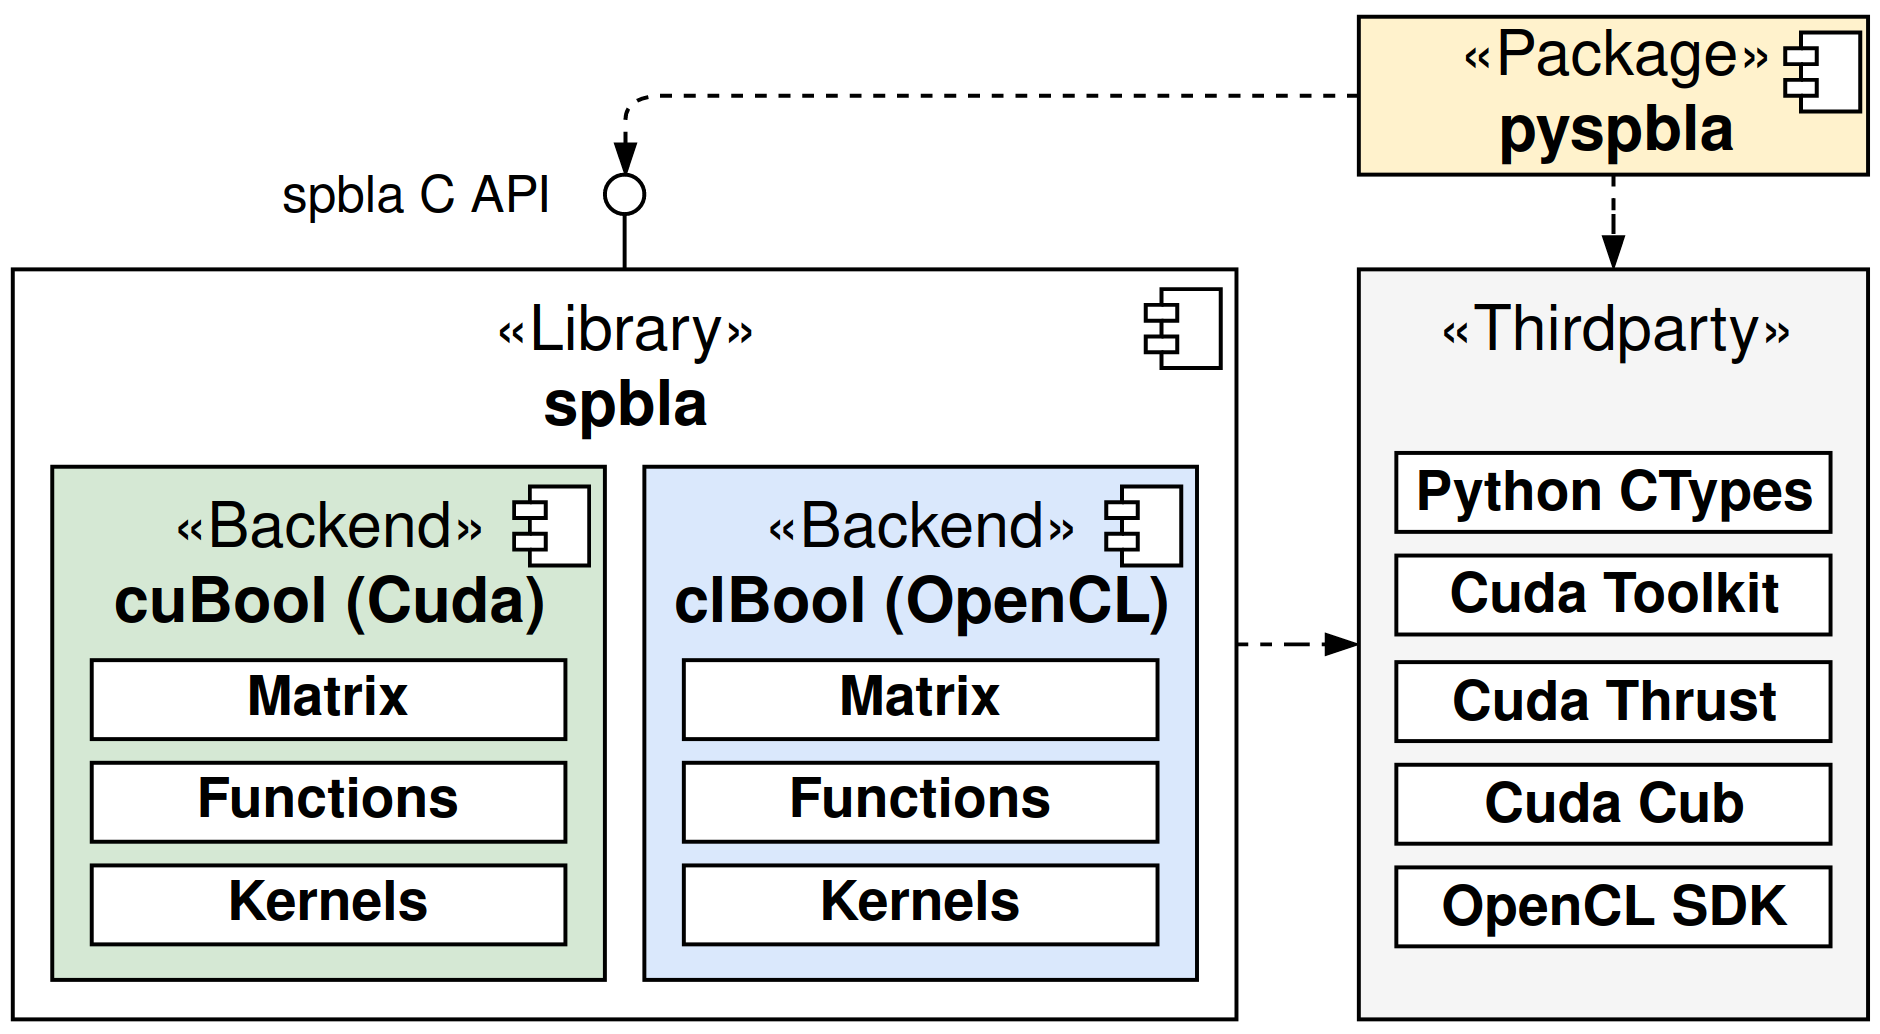
\includegraphics[width=0.39\textwidth]{generic_architecture.png}
    \caption{Sparse Boolean linear algebra libraries architecture.}
    \label{fig:generic_architecture}
\end{figure}

Libraries operate on the boolean semiring with values set \{\textit{true}, \textit{false}\} with \textit{false} as an identity element, '$+$' operation is defined as logical \textit{or} and '$\times$' is defined as logical \textit{and}.
Values are also denoted as $\{1,~0\}$ respectively, and the abbreviation $\textit{nnz(M)}$ gives the number of non-zero cells of the matrix $M$.

The main primitive is a sparse matrix of boolean values, stored in one of the sparse formats.
The sparse vector primitive is not supported, since it is rarely used in practical computational tasks.
Other available operations and functions are the following.

% \begin{itemize}
%     \item Create sparse matrix $M$ of size $m \times n$.
%     \item Delete sparse matrix $M$ and free all its internal resources.
%     \item Fill the matrix $M$ with values $L = \{(i,j)_k\}_k$. The result of this operation is $M_{i,j} = 1$ for each $(i, j) \in L$, and $M_{i,j} = 0$ otherwise.
%     \item \cho{Read matrix $M$ values $L = \{(i, j)~|~M_{i,j} = 1\}$.}
%     \item Matrix-matrix multiply-add operation $C \mathrel{+}= M \times N$.
%     \item Matrix-matrix add operation $M \mathrel{+}= N$.
%     \item Matrix-matrix Kronecker product $K = M \otimes N$.
% \end{itemize}

\begin{itemize}
    \item Create sparse matrix $M$ of size $m \times n$.
    \item Delete sparse matrix $M$.
    \item Fill matrix with values $\{(i,j)_k\}_k$.
    \item Read matrix values $\{(i, j)~|~M_{i,j} = 1\}$.
    \item Matrix-matrix multiplication $C \mathrel{+}= M \times N$.
    \item Matrix-matrix element-wise addition $M \mathrel{+}= N$.
    \item Matrix-matrix Kronecker product $K = M \otimes N$.
\end{itemize}
\section{Implementation Details}

Details on implementation. 

Architecture.
\section{Evaluation}

For performance analysis of proposed solution we evaluated some most common graph algorithms using real-world sparse matrix data. 
As a baseline for comparison we chose LAGraph~\cite{szarnyas2021lagraph} in connection with SuiteSparse~\cite{10.1145/3322125} as a CPU tool, Gunrock~\cite{7967137} and GraphBLAST~\cite{yang2019graphblast} as a Nvidia GPU tools. 
Also, we tested algorithms on several devices with distinct OpenCL vendors in order to validate portability of the proposed solution. 
In general, these evaluation intentions are summarized in the following research questions. 

\vspace{0.2cm}
\begin{itemize}
    \item[\textbf{RQ1}] What is the performance of the proposed solution relative to existing tools for both CPU and GPU analysis?
    
    \item[\textbf{RQ2}] What is the portability of the proposed solution with respect to various device vendors and OpenCL runtimes?
\end{itemize}

\subsection{Evaluation Setup}

For evaluation, we use a PC with Ubuntu 20.04 installed, which has 3.40Hz Intel Core i7-6700 4-core CPU, DDR4 64Gb RAM, and Nvidia GeForce GTX 1070 GPU with 8Gb VRAM. 
Host programs were compiled with GCC 9.3.0 compiler. Programs using CUDA were compiled with GCC 8.4.0 and Nvidia NVCC 10.1.243 compiler.
Release mode and maximum optimization level was enabled for all tested programs. 
Data loading time, preparation, format transformations and host-device initial communications are excluded from time measurements. 
All tests are averaged across 10 runs.
Additional warm-up run for each test execution is excluded from measurements.

\subsection{Graph Algorithms}

For preliminary study \textit{breadth-first search} (bfs) and \textit{triangles counting} (tc) algorithms were chosen, since they allows analyse the performance of \textit{vxm} and \textit{mxm} operations, rely heavily on \textit{masking}, and utilize \textit{reduction} or \textit{assignment}. 
BFS implementation utilizes automated vector storage from sparse to dense switch and only \textit{}{push optimization}. 
TC implementation uses masked \textit{mxm} of source lower-triangular matrix with second transposed argument.

\subsection{Dataset}

Nine graph matrices were selected from the Sparse Matrix Collection at University of Florida~\cite{dataset:10.1145/2049662.2049663}. 
Information about graphs is summarized in Table~\ref{dataset:info}. 
All datasets are converted to undirected graphs. 
Self-loops and duplicated edges are removed.

\begin{table}[htbp]
\caption{Dataset description.} 
\begin{center}
    \rowcolors{2}{black!2}{black!10}
    \begin{tabular}{|l|r|r|r|}
    \hline
    Dataset & Vertices  & Edges & Max Degree \\
    \hline
    \hline
    coAuthorsCiteseer & 227.3K &   1.6M &    1372 \\
    coPapersDBLP      & 540.4K &  30.4M &    3299 \\
    hollywood-2009    &   1.1M & 113.8M &  11,467 \\
    roadNet-CA        &   1.9M &   5.5M &      12 \\
    com-Orkut         &     3M &   234M &   33313 \\
    cit-Patents       &   3.7M &  16.5M &     793 \\
    rgg\_n\_2\_22\_s0 &   4.1M &  60.7M &      36 \\
    soc-LiveJournal   &   4.8M &  68.9M &  20,333 \\
    indochina-2004    &   7.5M & 194.1M & 256,425 \\
    \hline
    \end{tabular}
    \label{dataset:info}
\end{center}
\end{table}

\subsection{Results}

Table~\ref{results} presents results of the evaluation and compares performance of Spla against other tool on different execution platforms.
Tools are grouped by the type of the device for the execution, where either Nvidia GPU or Intel CPU are used. 
Cell left empty if tested tool failed to analyse graph due to \textit{out of memory} exception.

In general, Spla BFS shows acceptable performance, especially on graphs with large vertex degree, such as soc-LiveJournal and com-Orkut.
On graphs roadNet-CA and rgg it has a significant performance drop due to the nature of underlying algorithms and data structures. 
Firstly, library utilizes immutable data buffers. Thus, iteratively updated dense vector of reached vertices must be copied for each modification, what dominates the performance of the library on a graph with large search depth. 
Secondly, Spla BFS does not utilise \textit{pull optimization}, what is critical in a graph with relatively small search frontier. 

Spla TC has a good performance on GPU, which is better in all cases that reference SuiteSparse solution. 
But in most tests GPU competitors, especially Gunrock, show smaller processing times. 
GraphBLAST shows better performance as well. 
Library utilises masked SpGEMM algorithm, the same as in GraphBLAST, but without \textit{identity} element to fill gaps. 
Library explicitly stores all non-zero elements, and uses mask to reduce only non-zero while evaluating dot products of rows and columns. 
What causes extra divergence inside work groups. 
On Intel device Spla shows better performance compared to SuiteSparse on com-Orkut, cit-Patents and soc-LiveJournal. 
A possible reason is the large lengths of processed rows and columns in the product of matrices.

Gunrock shows nearly best average performance due to its specialized and optimized algorithms.
Also, it has good time characteristics on a mentioned earlier roadNet-CA and rgg in BFS algortihm. 
GraphBLAST follows Gunrock and show good performance as well. 
But it runs out of memory on a two significantly large graphs con-Orkut and indochina-2004. 
Spla does not rut out of memory on any test due to simplified storage scheme.

\begin{table}[htbp]
\caption{Graph algorithms evaluation results.\\Time in milliseconds (lower is better).} 
\begin{center}
    \begin{tabular}{|l|r|r|r|r|r|}
    \hline
    \multirow{2}{*}{Dataset} & \multicolumn{3}{c|}{Nvidia} & \multicolumn{2}{c|}{Intel} \\
    \cline{2-6}
    & GR & GB & SP & SS & SP \\
    \hline
    \hline
    \multicolumn{6}{|c|}{BFS} \\
    \hline
    \rowcolor{black!10} hollywood-2009    &  20.3 &  82.3 &   36.9 &   23.7 &   303.4 \\
    \rowcolor{black!2 } roadNet-CA        &  33.4 & 130.8 & 1456.4 &  168.2 &   965.6 \\
    \rowcolor{black!10} soc-LiveJournal   &  60.9 &  80.6 &   90.6 &   75.2 &  1206.3 \\
    \rowcolor{black!2 } rgg\_n\_2\_22\_s0 &  98.7 & 414.9 & 4504.3 & 1215.7 & 15630.1 \\
    \rowcolor{black!10} com-Orkut         & 205.2 & -- -- &  117.9 &   43.2 &   903.6 \\
    \rowcolor{black!2 } indochina-2004    &  32.7 & -- -- &  199.6 &  227.1 &  2704.6 \\
    \hline
    \hline
    \multicolumn{6}{|c|}{TC} \\
    \hline
    \rowcolor{black!10} coAuthorsCiteseer &   2.1 &    2.0 &    9.5 &    17.5 &    64.9 \\
    \rowcolor{black!2 } coPapersDBLP      &   5.7 &   94.4 &  201.9 &   543.1 &  1537.8 \\
    \rowcolor{black!10} roadNet-CA        &  34.3 &    5.8 &   16.1 &    47.1 &   357.6 \\
    \rowcolor{black!2 } com-Orkut         & 218.1 & 1583.8 & 2407.4 & 23731.4 & 15049.5 \\
    \rowcolor{black!10} cit-Patents       &  49.7 &   52.9 &   90.6 &   698.3 &   684.1 \\
    \rowcolor{black!2 } soc-LiveJournal   &  69.1 &  449.6 &  673.9 &  4002.6 &  3823.9 \\
    \hline
    \hline
    \multicolumn{6}{l}{Tools: Gunrock (GR), GraphBLAST (GB), SuiteSparse (SS), Spla (SP).} \\
    \end{tabular}
    \label{results}
\end{center}
\end{table}
 
% Two GPU

% \begin{table}[htbp]
%     \caption{Table Type Styles}
%     \begin{center}
%     \begin{tabular}{|c|c|c|c|}
%     \hline
%     \textbf{Table}&\multicolumn{3}{|c|}{\textbf{Table Column Head}} \\
%     \cline{2-4} 
%     \textbf{Head} & \textbf{\textit{Table column subhead}}& \textbf{\textit{Subhead}}& \textbf{\textit{Subhead}} \\
%     \hline
%     copy& More table copy$^{\mathrm{a}}$& &  \\
%     \hline
%     \multicolumn{4}{l}{$^{\mathrm{a}}$Sample of a Table footnote.}
%     \end{tabular}
%     \label{tab2}
%     \end{center}
% \end{table}

\section{Conclusion}

In this paper we present a library for sparse Boolean linear algebra which implements such basic operations as matrix-matrix multiplication and element-wise matrix-matrix addition in both Cuda and OpenCL.
Evaluation shows that our Boolean-specific implementations faster and require less memory than generic, not the Boolean optimized, operations from state-of-the-art libraries. 
Thus, the specialization of operations for this data type makes sense. 

The first direction of the future work is to integrate all parts (OpenCL and Cuda backends) into a single library and improve its documentation and prepare to publish.
Moreover, it is necessary to extend the library with other operations, including matrix-vector operations, masking, and so on.
As a result a Python package should be published.

Another important step is to evaluate the library on different algorithms and devices.
Namely, algorithms for RPQ and CFPQ should be implemented and evaluated on related data sets.
Also, it is necessary to evaluate OpenCL version on FPGA which may require additional technical effort and code changes.

Finally, we plan to discuss with GraphBLAS community possible ways to use our library as a backend for GraphBLAST or SuiteSparse in case of Boolean computations.
Moreover, it may be possible to use implemented algorithms as a foundation for generalization to arbitrary semirings.

\section{Appendix}

Project page \href{https://github.com/JetBrains-Research/spla}{https://github.com/JetBrains-Research/spla}.

%\section*{Acknowledgment}
%
%The preferred spelling of the word ``acknowledgment'' in America is without
%an ``e'' after the ``g''. Avoid the stilted expression ``one of us (R. B.
%G.) thanks $\ldots$''. Instead, try ``R. B. G. thanks$\ldots$''. Put sponsor
%acknowledgments in the unnumbered footnote on the first page.


\bibliographystyle{./IEEEtran}
\bibliography{./Sparse_Boolean_Algebra_on_GPGPU}

\end{document}
